\chapter{Problem Analysis}
\label{s:analy}
This chapter provides a thorough analysis of the data stream provided by the camera, and of the objects displayed therein.
We discuss the anatomy of human face and eyes in particular, and all relevant technical details about commonly used web cameras.

\section{Conditions}

We expect that the user is working with their personal computer or a similar device such as a tablet.
The user and the device can freely move around; the only constraint there is that the camera must be fixed to the computer screen.

\begin{figure}[h]
	\centering 
	\centering 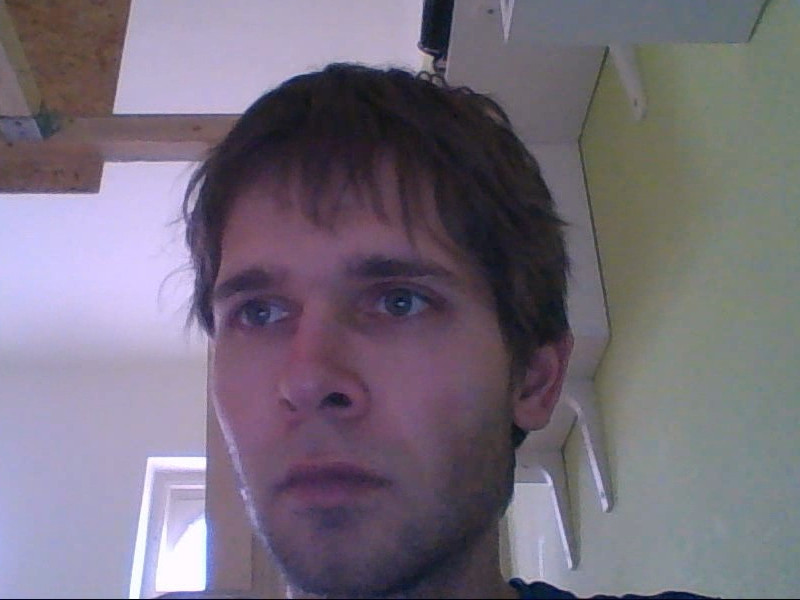
\includegraphics[width=0.7\linewidth]{img/analy-shot.jpg}
	\caption{Example input frame (see Attachment \ref{s:testingdata}).}\label{i:analy-shot}
\end{figure}

Throughout the computation, we rely on that the user's face and both eyes are visible, and that the angle difference of the gaze and the camera direction is small.
We do not impose any further constraints on the face pose relatively to the camera.
For example, it is not necessary that the camera be upright, since some users might find it more comfortable to attach a camera to the bottom of their screen upside down.
Such a constraint could also pose a difficulty for users working with a vertically rotated screen.

For a good calibration, we require active cooperation from the user: they are asked to watch a dot moving around the screen.
If necessary, this requirement can be somewhat lifted by using a calibration file defined earlier or by some completely different means of calibration.
We allow the user to move their head but we cannot actually rely on this because many users (e.g. disabled ones) may have difficulties to move.

Ambient lighting must be good enough for the camera to deliver a high-contrast and sharp image.
The image brightness, white balance etc. are allowed to change abruptly and always.
There is, however, a strong requirement on the light being rather diffuse than directional, and making no sharp shadows on the user's face.
If the light conditions substantially start to differ from the ones during calibration, it may be necessary to re-calibrate.

Cluttered environment is not an issue as long as the extraneous objects do not occlude the view and do not oversaturate (dazzle) the camera.
An example of what the input image could look like is given in Figure ref{i:analy-shot}.

\section{Human head}

We consider it important to introduce some basic terms and facts about human anatomy in order to better understand the problem at hand.

\begin{figure}[ht]
	\centering 
	\begin{subfigure}[b]{0.55\textwidth}
		\centering 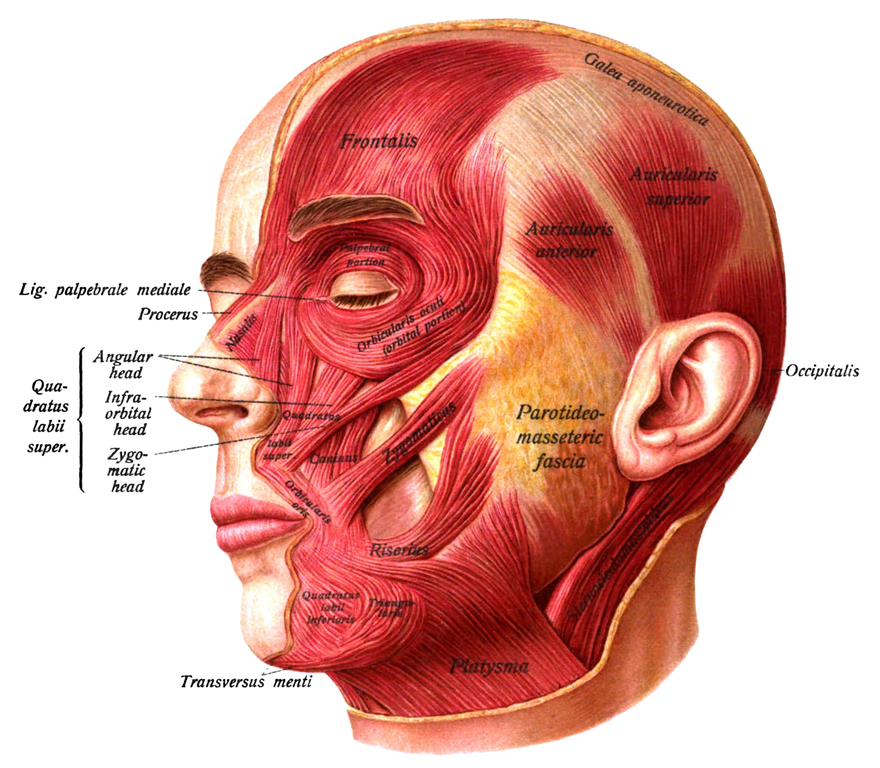
\includegraphics[width=\linewidth]{img/analy-face.png} \caption{Human face. (J. Sobota, public pomain)} \label{i:analy-face}
	\end{subfigure}
	\begin{subfigure}[b]{0.44\textwidth}
		\centering 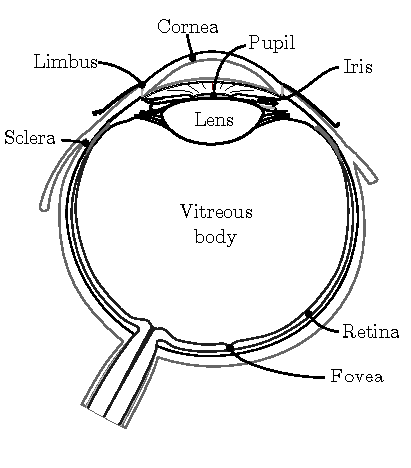
\includegraphics[width=\linewidth]{img/analy-eye.pdf}
		\caption{Human eye. (Adopted from \href{https://commons.wikimedia.org/wiki/File:Schematic_diagram_of_the_human_eye_en.svg}{\tt commons.wikimedia.org}, CC0)}\label{i:analy-eye}
	\end{subfigure}
	\caption{Illustration of an undesired result of the Poisson reconstruction.}\label{i:analy-anatomy}
\end{figure}

\subsection{Face anatomy}
The face is the frontal part of human head.
Facial muscles are specific in that they are attached to the skin, and their almost sole purpose is communication.
As seen in Figure \ref{i:analy-face}, there is hardly a spot on the face that would not have muscles underneath.
Although they can be controlled by will, they often actuate subconsciously.
There are kinds of subtle movements, usually induced by basic emotions such as fear, that can not be prevented by will.
In a summary, the facial skin is flexible with a virtually infinite number of degrees of freedom, and almost its whole area is controlled by muscles.

Of special interest for us are regions that remain mostly fixed to the skull in normal conditions.
These include the nose (especially its upper part), the chin and small outer regions around and slightly below the eyes.
The chin is very prominent and easy to track, but may become completely misleading if the user opens their mouth.
Given the flexibility discussed above, it is almost impossible to estimate head pose precisely, but we can get a good estimate by choosing some of these less expressive regions.

The face also contains many features that hinder gaze recognition.
Typically, people keep their eyelids open just quite enough so as not to occlude the pupil.
This poses a serious challenge to all techniques based on the iris: in many people, only about half of the iris area is visible.

On the edges of eyelids there are eyelashes.
Depending on the viewing angle, these can also significantly occlude the eye.
As if this all was not enough, the user may wear strong makeup and a mascara to emphasize these undesirable factors.

Assistive tools like glasses and contact lenses also have to be considered when designing a gaze tracker, although they are technically not a part of the face.
Glasses and lenses (including the natural ones) will cause an unpredictable displacement of the iris and pupil image.
A flexible enough gaze estimator may be capable of handling this distortion implicitly.
In fact, glasses with solid rims can help head pose estimation as their position relatively to the skull remains reliably constant.

\subsection{Eye anatomy}
\label{s.eyeanatomy}

The eyeball consists of several functional parts.
The most notable ones are depicted in Figure \ref{i:analy-eye}:
\begin{itemize}
\item Transparent \textit{cornea}, a fixed lens also providing some mechanical protection
\item Flexible and reflective \textit{iris}, which serves as a diaphragm
\item Flexible \textit{lens} stretched by several muscles to control its optical magnitude
\item Purely white \textit{sclera}, which serves as a hard shell of the eyeball
\item \textit{Vitreous body}, a transparent gel to maintain the inner pressure
\item Light-sensitive \textit{retina}
\end{itemize}

Furthermore, each eyeball is embedded in a hole called the \textit{orbit} that provides fixation and actuation.
There are six separately controlled muscles stretching between to the eyeball and the orbit.

Throughout the literature, eye is modeled either as a sphere \cite{zhang13}, or with an extra spherical section for the cornea \cite{villanueva08}.
Some sources, such as \cite{wang16}, also explicitly model the eyelids.

The sclera of human eye is made of white collagen.
The color of the iris, in turn, can vary anywhere between bright blue and dark brown, including some less common shades like green and amber.
It feels quite intuitive that these distinctive colors have evolved for the purposes of nonverbal communication.
This claim is known as the \textit{cooperative eye hypothesis} and has been, in part, proven by experiment \cite{tomasello07}.

In addition, the aperture inside the iris, known as the \textit{pupil}, displays the retina through the lens.
The retina absorbs light in order to acquire as much information as possible, and therefore it is mostly black.
A notable exception is the red-eye effect that may appear in directional light.
Its usefulness to eye tracking has been discussed in Section \ref{s:related-gazetracking}, but since we assume diffuse lighting, this effect should not be present.

The inner and outer boundary of the human iris (the pupil and the limbus, respectively) are concentric circles.
Generally, the inner shape of the iris is the less reliable of these two.
An extreme case is when the pupil is permanently distorted and non-circular due to a damage \cite[p.5]{bowyer16} or a disease \cite[p.146]{bowyer16}.

In healthy people, the radius of the pupil changes depending on the amount of incoming light and on their emotional state.
The constriction is controlled by the parasympathicus, a nervous system generally related to comfortable actions such as eating and sleeping.
The dilation is controlled by the sympathicus, which in turn is the main actuator of the ``fight or flight" stress response.
Both the sympathicus and parasympathicus are parts of the autonomous nervous system and as suggested by the name, they cannot be directly controlled by will.

\subsection{Eye movement}

When attending to an object (or another person), people will automatically turn their eyes directly towards it.
This process is usually subconscious and some of its aspects are involuntary.

The main reason for eye movement is that the overall acuity of our visual system increases towards a small area near the optical axis.
The corresponding spot on the retina is called the \textit{fovea}, and it is located about $5\degree$ off-axis horizontally towards the nose \cite{villanueva08}.
It covers only about $1.5\degree$ of the visual field.
The density of photopic (daylight-sensitive) cells in the fovea is up to 20 times more than in the peripheral areas of the retina.

Although gaze can be precisely controlled by will, there are many peculiarities about eye motion that depend on old brain circuitry and are common to all humans.

Assuming that each muscle can apply force only by stretching, and not extending itself, the six muscles provide three degrees of freedom (DoF) to the eye motion---but only two DoF are necessary to control the gaze direction.
A third DoF, namely rotation around the optical axis (the \textit{roll}) is actively used by the brain.
The effect is slight, but because fovea is offset from the optical axis, this could make the gaze direction unpredictable given the optical axis only.
Fortunately, the roll is deterministic with respect to the remaining two rotation angles.
This fact is known as the \textit{Donder's Law} \cite{hansen10}, and thanks to it, the effect of eye roll can be implicitly precalculated during calibration.

The gaze is usually controlled by high-level brain regions automatically so as to observe all necessary details about the environment.
This process is mainly based on visual feedback, and can be predicted to an extent by simple image processing, such as in \cite{yucel09}.
There are three basic actions that our visual system is capable of: a \textit{saccade}, a \textit{fixation}, and a \textit{smooth pursuit}.

The purpose of saccades is to point the gaze in a new direction.
During eye movement, the visual input is distorted by motion blur, so it is desirable that it be as quick as possible.
Indeed, the angular acceleration in the beginning and in the end of a saccade reaches the order of $\num{10000}\degree/\mathrm{s}^2$
The periods when the eye is static are called fixations.

\begin{figure}[h]
	\centering 
	\centering 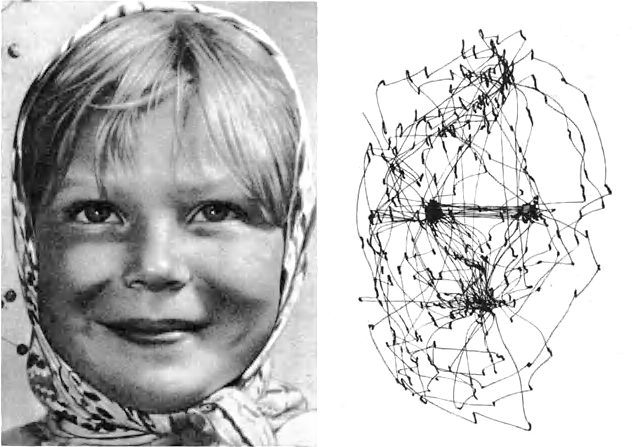
\includegraphics[width=0.7\linewidth]{img/analy-saccade.png}
	\caption{Gaze recording. (L. Yarbus \cite{yarbus67})}\label{i:analy-saccade}
\end{figure}

It is important to note that what we feel like a constant gaze direction is actually a sequence of saccades and fixations.
Although a single fixation may suffice to identify an object, the whole visual system relies on its ability to perform saccades constantly.
The scale of these saccades varies greatly, a microsaccade measured in an experiment can be considered small within the fixation threshold in another one.
For a rough estimate, we can say that the eye moves less than $1\degree$ during a fixation.
This corresponds to the $1.5\degree$ diameter of the fovea: when attending to an object, it is enough to project it quite anywhere on the fovea, in order to get a good image.
Figure \ref{i:analy-saccade} shows a sequence of saccades and fixations as recorded when viewing a static image for three minutes.

Our tracker will ignore these details about eye motion since they are much below the expected resolution of our program.
It is important to remember, though, that the speed of saccades makes the gaze very unpredictable.
For example, it would not be wise to impose a maximum gaze offset relatively to the previous known position.

Finally, there is a special kind of eye movement for following objects that actually move around.
This is referred to as the smooth pursuit, and it is characterized by a smooth, saccade-less eye movement.

People are usually unable to perform smooth pursuit without a moving object in sight.
On the other hand, if a moving target is drawn on the screen with a low frame rate, our perception of it will be blurry because the eye will traverse a smooth path during each frame.
Being so predictable and precise, smooth pursuit is perfect for the calibration of a gaze tracker.

\section{Gaze}
\label{s:gaze-model}

The gaze is the direction of focus of the user.
We assume that it is a ray originating in the eye, and that its direction is unambiguously given by the eye rotation.
Furthermore, we expect the ray be pointed to somewhere on the computer screen.
The typical setting is drawn out in Figure \ref{i:analy-gaze}.

\begin{figure}[h]
	\centering 
	\centering 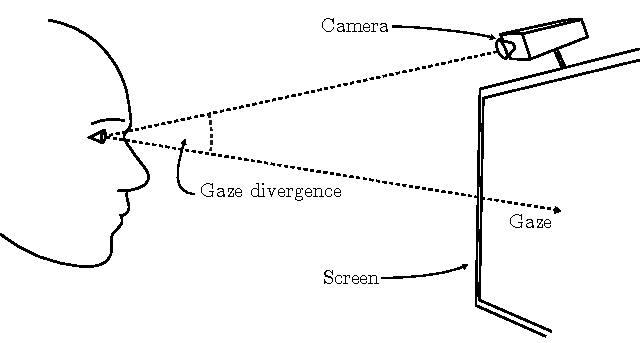
\includegraphics{img/analy-gaze.pdf}
	\caption{Sketch of the scene.}\label{i:analy-gaze}
\end{figure}

Gaze is affected by both the head pose and eye rotation.
Although it may seem more efficient to only move our eyes when using a computer, people usually move their heads quite a lot.
In fact, prolonged static pose of the head can cause pain in the spine.

There are no strict constraints regarding the scene configuration.
Perhaps the only requirement is our assumption of small angle divergence.
The gaze angle when the user looks directly into the camera and when they look to the farthest point on the screen should not differ by more than about $30\degree$.
This means that the iris can be anisotropically stretched by a factor of about $0.9$, which can still be approximated as a circle.\footnote{
Assuming that the camera lies in the screen plane, this factor equals $\mathrm{cos}(30\degree) \approx 0.87$.
}

We model movement of the iris as a simple translation.
It should be clear that because the head and the eyes differ by an order of magnitude in scale, gaze estimation is numerically unstable.
A small variation in the eye rotation induces an even smaller variation in the iris position, but may correspond to a large change of gaze.

We avoid explicit modeling of the viewed scene by assuming that the gaze is given by a homography, as it will be detailed in Section \ref{s:impl-gaze}.

\section{Camera}

A suitable yet very simple mathematical model of a video camera is the pinhole camera.
Light rays passing through a certain point in space (figuratively, the pinhole) are projected onto an image plane.
The axis of symmetry of this system is called the optical axis, and the intersection of the optical axis with the image plane is assumed to be the origin point in image coordinates.

Real-world cameras can suffer from many kinds of degeneracies off this model:
\begin{itemize}

\item
Imprecise manufacturing.
The image origin point may be offset from the optical axis.
The sensor may be stretched and skewed, so that orthonormal vectors in image plane are not always sensed as orthonormal.

\item
Blur.
Refractive lens are usually inserted into the optical path so that light need not pass through an infinitely small pinhole, but rather though a small disc.
This approach results in that only light rays originating from a certain surface in the scene, known as the focal plane, are properly projected onto the image plane.
Points from a plane parallel with the focal plane will be displayed as if convolved with a disc kernel; the radius increases with the parallel distance from the focal plane, and the shape is mostly a projection of the camera iris.

The lens may be dirty or scratched, which casues a slight and uniform foggy blur.
In very small cameras with relatively high resolution, the wave nature of light may cause additional blur by diffraction at edges of the camera iris.

\item
Lens aberration.
The lens itself is a thick solid object and therefore can never fulfill its physical model perfectly.
The nonlinear effect usually manifests itself by stretching sensed points in or out relatively to the image origin point.
If carefully measured, this geometric transformation within the image plane can be very well cancelled.

Because the refractive index of materials varies with wavelength (this fact is known as dispersion), the nonlinearities are also wavelength dependent.
There are software tools to reduce percieved color aberration, but this problem is under-determined and can never be solved exactly.
A proper solution would require to densely sample the spectrum at each image point but we only have three values roughly corresponding to red, green and blue.

These effects are often well compensated in high-end cameras by sophistication of the optical system.
On the other hand, they also decrease with the lens size, and cameras with a narrow or almost closed iris can be fairly well aproximated as pinhole cameras with no lens.

\item
Moiré.
In most consumer cameras, image colors are obtained by attaching a color filter in front of the sensor, so that each light-sensitive element receives either red, green or blue light only.
These colors are interleaved in a fine pattern.
Color pixel can be obtained from each element by looking at two neighbors neighbors that have different filters, in the hope these neighbors are lit by roughly the same color.
Alas, contrast on subpixel level makes each of these color sensors receive a different amount of light, even if there are no actual colored objects in the scene.
When imaging fine black-and-white colored structures, spurious and highly saturated colors may appear.

This effect can hardly occur when displaying human faces.
Quite to the contrary, it can be used for manual focusing of the camera, if necessary.
Moiré is an optical effect between the imaged object and the light sensor, and usually will not be affected by image processing such as denoising algorithms.
We can put a black and white grid nearby the user's head and tune the camera focus until color moiré appears.

\end{itemize}

\section{Image}
\label{s.imagemodel}

The image acquired from the camera is a rectangular grid of colored points, expressed as a matrix $\mat M \in \R^{n\times m}$.
However, certain parts of the computation require a continuous image model in order to obtain a sub-pixel precision.
In such cases, the image function is defined by bilinear interpolation:
\begin{align}
\f{I}(\vec p, \mat M) = (1 - t) \cdot&\left((1 - s) \mat M_{i, j} + s \cdot \mat M_{i, j+1} \right) \\
+ t&\left((1 - s) \mat M_{i+1, j} + s \cdot \mat M_{i+1, j+1} \right), \notag
\end{align}
where $\vec p = (i + t, s + j)\T$, $s, t \in \lbrack0, 1)$ and $i, j$ are whole numbers.

The partial derivatives of an image are approximated as
\begin{equation}
\f I_x(\vec p, \mat M) = \f I\left((\vec p_1 - \frac 1 2, \vec p_2)\T, \mat D\right),
\end{equation}
where $\mat D_{i, j} = \mat M_{i,j+1} - \mat M_{i, j}$.

Note that each derivative is sampled at a slightly shifted position.
While this may seem needlessly picky, precise coordinates become very important when working with the image pyramid in Section \ref{s:impl-face}.
A half-pixel shift in a downscaled image can represent a very large distance in the original pixel grid, and ignoring this displacement would actually make our algorithms fail.

Nevertheless that the bilinear interpolation is an attractive choice, it does not produce a smooth function.
We shall need to interpolate not only the image but also its derivatives up to the second order.
In general, this problem has three possible solutions.

Firstly, we can interpolate both the image and its discretely evaluated derivatives using a simple formula, and ignore the inaccuracy induced.
This is the approach applied in this thesis.

The second option is to use such simple interpolation on a blurred image in the hope that the inaccuracy disappears.
This solution is implicitly used by many software libraries.

Finally, it is possible to interpolate using a sophisticated filter such as the Lanczos function $\f{sinc}(x) \cdot \f{sinc}(x/2), x \in (-2, 2)$.
Both its first and second derivatives are continuous and bounded within $(-1, 1)$.
The problem is that they are prohibitively hard to calculate.
In the end, this may lead us to only estimating these derivatives by a simple formula---but by making such a step, we effectively classify to the first category above.
